\documentclass[12pt, titlepage]{article}

\usepackage{booktabs}
\usepackage{tabularx}
\usepackage{hyperref}
\usepackage{float}
\usepackage{graphicx}
\usepackage{float}
\usepackage[letterpaper, portrait, margin=1in]{geometry}
\usepackage{helvet}
\hypersetup{
    colorlinks,
    citecolor=black,
    filecolor=black,
    linkcolor=red,
    urlcolor=blue
}
\usepackage[round]{natbib}
\graphicspath{ {./docs/VNVReport} }
\renewcommand{\familydefault}{\sfdefault}
%% Comments

\usepackage{color}

\newif\ifcomments\commentstrue %displays comments
%\newif\ifcomments\commentsfalse %so that comments do not display

\ifcomments
\newcommand{\authornote}[3]{\textcolor{#1}{[#3 ---#2]}}
\newcommand{\todo}[1]{\textcolor{red}{[TODO: #1]}}
\else
\newcommand{\authornote}[3]{}
\newcommand{\todo}[1]{}
\fi

\newcommand{\wss}[1]{\authornote{blue}{SS}{#1}} 
\newcommand{\plt}[1]{\authornote{magenta}{TPLT}{#1}} %For explanation of the template
\newcommand{\an}[1]{\authornote{cyan}{Author}{#1}}

%% Common Parts

\newcommand{\progname}{ProgName} % PUT YOUR PROGRAM NAME HERE
\newcommand{\authname}{Team \#, Team Name
\\ Student 1 name and macid
\\ Student 2 name and macid
\\ Student 3 name and macid
\\ Student 4 name and macid} % AUTHOR NAMES                  

\usepackage{hyperref}
    \hypersetup{colorlinks=true, linkcolor=blue, citecolor=blue, filecolor=blue,
                urlcolor=blue, unicode=false}
    \urlstyle{same}
                                


\begin{document}

\title{Verification and Validation Report: \progname} 
\author{\authname}
\date{\today}
	
\maketitle

\pagenumbering{roman}

\section{Revision History}

\begin{tabularx}{\textwidth}{p{3cm}p{2cm}X}
\toprule {\bf Date} & {\bf Version} & {\bf Notes}\\
\midrule
Date 1 & 1.0 & Notes\\
Date 2 & 1.1 & Notes\\
\bottomrule
\end{tabularx}

~\newpage

\section{Symbols, Abbreviations and Acronyms}

\renewcommand{\arraystretch}{1.2}
\begin{tabular}{l l} 
  \toprule		
  \textbf{symbol} & \textbf{description}\\
  \midrule 
  T & Test\\
  \bottomrule
\end{tabular}\\

\wss{symbols, abbreviations or acronyms -- you can reference the SRS tables if needed}

\newpage

\tableofcontents

\listoftables %if appropriate

\listoffigures %if appropriate

\newpage

\pagenumbering{arabic}

This document ...

\section{Functional Requirements Evaluation}

\section{Nonfunctional Requirements Evaluation}

\subsection{Usability}
		
\subsection{Performance}

\subsection{etc.}
	
\section{Comparison to Existing Implementation}	

Current motion detecting smart watches, such as Apple watches or Samsung Galaxy watches, are desgined for healthy and active population. The EMAnator is specifically geared towards older adults who have chronical back pain. Therefore, it is desgined to capture minor and subtle movements accurately.

\section{Unit Testing}

\begin{center}
\begin{table} 
\begin{tabular}{ | p{0.5cm} | p{2.8cm} |  p{1.1cm} | p{2.7cm} | p{2.7cm} | p{2.7cm} | p{1.1cm} |}
\hline
\textbf{No.} & \textbf{Name}  & \textbf{Ref.} & \textbf{Action} & \textbf{Expected Output} & \textbf{Actual Output} & \textbf{Result} \\
\hline
 1 & bed\_HR\_setup & \href{https://github.com/zakerl/Capstone_Project/blob/main/docs/SRS/SRS.pdf}{R2} & Power on the device. & "PulseSensor object created", LED flash per each heartbeat. & "PulseSensor object created", LED flash per each heartbeat. & Pass \\ 
\hline
2 & bed\_HR\_detect & \href{https://github.com/zakerl/Capstone_Project/blob/main/docs/SRS/SRS.pdf}{R2} & Walk for 10 seconds while wearing the device, then stop. & "HeartBeat Detected. BPM: 70”. & "HeartBeat Detected. BPM: 130”. & Fail \\  
\hline
3 & bed\_MPU\newline \_setup & \href{https://github.com/zakerl/Capstone_Project/blob/main/docs/SRS/SRS.pdf}{R2} & Power on the device. & “Calibrating MPU in 4 seconds! Hold it still! avg X acc: 20, , avg Y acc: 20, avg Z acc: 20” & “Calibrating MPU in 4 seconds! Hold it still! avg X acc: 20, , avg Y acc: 20, avg Z acc: 20” & Pass \\  
\hline
4 & bed\_MPU\newline \_detect & \href{https://github.com/zakerl/Capstone_Project/blob/main/docs/SRS/SRS.pdf}{R2} & Limp & “limp count + limp count + limp count + limp count + limp count + limping. Stepcount: 5” & “limp count + limp count + limp count + limp count + limp count + limping. Stepcount: 5” & Pass \\ 
\hline
5 & bed\_init\_display & \href{https://github.com/zakerl/Capstone_Project/blob/main/docs/SRS/SRS.pdf}{NFR2} & Action & Black screen on & Black screen on & Pass \\ 
\hline
6 & bed\_scroll\_test &  \href{https://github.com/zakerl/Capstone_Project/blob/main/docs/SRS/SRS.pdf}{NFR2} & Scroll through 2 bezels in counter clock-wise direction. & Selection goes up. & Selection goes up. & Pass \\ 
\hline
7 & bed\_splash\newline \_screen & \href{https://github.com/zakerl/Capstone_Project/blob/main/docs/SRS/SRS.pdf}{NFR2} & Power on the device. & "Back End Developers" & "Back End Developers" & Pass \\ 
\hline
8 & bed\_display\newline \_one\_line & \href{https://github.com/zakerl/Capstone_Project/blob/main/docs/SRS/SRS.pdf}{NFR2} & Select a response for generated prompt & Screen clears prompt list and only displays current date and time. & Screen clears prompt list and only displays current date and time. & Pass \\ 
\hline
9 & OpenFile & \href{https://github.com/zakerl/Capstone_Project/blob/main/docs/SRS/SRS.pdf}{R6} & Press button and choose the "data.txt" file. & Contents of "data.txt" is displayed on UI. & Contents of "data.txt" is displayed on UI.  & Pass \\ 
\hline
\end{tabular}
\end{table}
\end{center}

\begin{center}
\begin{table} 
\begin{tabular}{ | p{0.5cm} | p{2.8cm} |  p{1.1cm} | p{2.7cm} | p{2.7cm} | p{2.7cm} | p{1.1cm} |}
\hline
\textbf{No.} & \textbf{Name}  & \textbf{Ref.} & \textbf{Action} & \textbf{Expected Output} & \textbf{Actual Output} & \textbf{Result} \\
\hline
10 & bed\_display\newline \_prompt & \href{https://github.com/zakerl/Capstone_Project/blob/main/docs/SRS/SRS.pdf}{R3} & Move around for 5 seconds and then stop for 5 seconds. & "Are you in pain?", Yes, No & "Are you in pain?", Yes, No & Pass \\ 
\hline
11 & bed\_format\newline \_prompt & \href{https://github.com/zakerl/Capstone_Project/blob/main/docs/SRS/SRS.pdf}{R3} & Limp with the device to activate prompt generation. & Prompt text color is white while background is black. & Prompt text color is white while background is black.  & Pass \\ 
\hline
12 & OpenSerial & \href{https://github.com/zakerl/Capstone_Project/blob/main/docs/SRS/SRS.pdf}{R6, NFR14} & Connect device to computer via USB port. & UI displays green dot. & UI displays green dot. & Pass \\ 
\hline
13 & bed\_init\_rtc & \href{https://github.com/zakerl/Capstone_Project/blob/main/docs/SRS/SRS.pdf}{R6, NFR1} & Power on the device. & "March 5th, 16:21". & "March 5th, 16:21". & Pass \\ 
\hline
14 & bed\_display\_info & \href{https://github.com/zakerl/Capstone_Project/blob/main/docs/SRS/SRS.pdf}{NFR2} & Power on the device. & "March 5th, 16:23". & "March 5th, 16:23". & Pass \\ 
\hline
15 & bed\_set\newline \_explicit\_date\newline \_time & \href{https://github.com/zakerl/Capstone_Project/blob/main/docs/SRS/SRS.pdf}{R6, NFR1} & Disconnect power source, reconnect, and power on the device. & "March 5th, 16:46". & "March 5th, 16:46". & Pass \\ 
\hline
16 & bed\_touch\newline \_detect & \href{https://github.com/zakerl/Capstone_Project/blob/main/docs/SRS/SRS.pdf}{NFR2} & Touch 2 bezels in clockwise direction. & 1 & 1 & Pass \\ 
\hline
17 & \_\_init\_\_ & N/A & Run the host software. & Login page appears. & Login page appears. & Pass \\ 
\hline
18 & saveAsTxt & \href{https://github.com/zakerl/Capstone_Project/blob/main/docs/SRS/SRS.pdf}{R6} & Press Save as button and choose a directory to save file in. & Config.txt file created and saved. & Config.txt file created and saved. & Pass \\ 
\hline
19 & BackToMain & \href{https://github.com/zakerl/Capstone_Project/blob/main/docs/SRS/SRS.pdf}{NFR2} & Press the main button. & Main screen appears and current screen closes. & Main screen appears and current screen closes. & Pass \\ 
\hline
20 &  InsertDB & \href{https://github.com/zakerl/Capstone_Project/blob/main/docs/SRS/SRS.pdf}{R6, NFR14} & Press save button. & Data appears on database table. & Data appears on database table. & Pass \\ 
\hline
\end{tabular}
\end{table}
\end{center}

\begin{center}
\begin{table} 
\begin{tabular}{ | p{0.5cm} | p{2.8cm} |  p{1.1cm} | p{2.7cm} | p{2.7cm} | p{2.7cm} | p{1.1cm} |}
\hline
\textbf{No.} & \textbf{Name}  & \textbf{Ref.} & \textbf{Action} & \textbf{Expected Output} & \textbf{Actual Output} & \textbf{Result} \\
\hline
21 & LoadDb & \href{https://github.com/zakerl/Capstone_Project/blob/main/docs/SRS/SRS.pdf}{R6, NFR14} & Press load button. & Data appears on software UI table. &  Data appears on software UI table. & Pass \\ 
\hline
22 & dataHead & \href{https://github.com/zakerl/Capstone_Project/blob/main/docs/SRS/SRS.pdf}{R6, NFR14} & Press load button. & Data appears on software UI table. & Data appears on software UI table. & Pass \\ 
\hline
23 & search & \href{https://github.com/zakerl/Capstone_Project/blob/main/docs/SRS/SRS.pdf}{R6, NFR14} & Filter-search participant first name of “John” & All participant record with first name “John” appears. & All participant record with first name “John” appears. & Pass \\ 
\hline
24 & OpenGraph & \href{https://github.com/zakerl/Capstone_Project/blob/main/docs/SRS/SRS.pdf}{R7} & Press graph button. & Empty graph chart appears. & Empty graph chart appears. & Pass \\ 
\hline
25 & OpenHeart & \href{https://github.com/zakerl/Capstone_Project/blob/main/docs/SRS/SRS.pdf}{R7} & Press heart rate button. & Only heart rate graph appears. & Only heart rate graph appears. & Pass \\ 
\hline
26 & OpenSteps & \href{https://github.com/zakerl/Capstone_Project/blob/main/docs/SRS/SRS.pdf}{R7} & Press steps button. & Only number-of-steps graph appears. & Only number-of-steps graph appears. & Pass \\ 
\hline
27 & OpenActivity & \href{https://github.com/zakerl/Capstone_Project/blob/main/docs/SRS/SRS.pdf}{R7} & Press activity button & Only activity graph appears. & Only activity graph appears. & Pass \\ 
\hline
28 & plot & \href{https://github.com/zakerl/Capstone_Project/blob/main/docs/SRS/SRS.pdf}{R7} & Press steps button. & Only number-of-steps graph appears. & Only number-of-steps graph appears. & Pass \\ 
\hline
29 & loginAttempt & \href{https://github.com/zakerl/Capstone_Project/blob/main/docs/SRS/SRS.pdf}{NFR8, NFR14} & ID: "admin", PW: "capstone" & Main screen appears. & Main screen appears. & Pass \\ 
\hline
30 & loginAttempt & \href{https://github.com/zakerl/Capstone_Project/blob/main/docs/SRS/SRS.pdf}{NFR8, NFR14} & ID: "wr1ong", PW: "creden5tials" & "Wrong credentials!" & "Wrong credentials!" & Pass \\ 
\hline
31 & showRecord\newline Window & \href{https://github.com/zakerl/Capstone_Project/blob/main/docs/SRS/SRS.pdf}{NFR2} & Press records button. & Records window appears and main window closes. & Records window appears and main window closes. & Pass \\ 
\hline
32 & showCreate\newline Records & \href{https://github.com/zakerl/Capstone_Project/blob/main/docs/SRS/SRS.pdf}{NFR2} & Press create records button. & Create Records window appears and main window closes. & Create Records window appears and main window closes. & Pass \\ 
\hline
\end{tabular}
\end{table}
\end{center}

\begin{center}
\begin{table} 
\begin{tabular}{ | p{0.5cm} | p{2.8cm} |  p{1.1cm} | p{2.7cm} | p{2.7cm} | p{2.7cm} | p{1.1cm} |}
\hline
\textbf{No.} & \textbf{Name}  & \textbf{Ref.} & \textbf{Action} & \textbf{Expected Output} & \textbf{Actual Output} & \textbf{Result} \\
\hline
33 & showConfig\newline View & \href{https://github.com/zakerl/Capstone_Project/blob/main/docs/SRS/SRS.pdf}{NFR2} & Press configuration button. & Configuration window appears and main window closes. & Configuration window appears and main window closes. & Pass \\ 
\hline
34 & showDataView & \href{https://github.com/zakerl/Capstone_Project/blob/main/docs/SRS/SRS.pdf}{NFR2} & Press data view button. & Data view window appears and main window closes. & Data view window appears and main window closes. & Pass \\ 
\hline
\end{tabular}
\end{table}
\end{center}

\section{Changes Due to Testing}

After testing out each unit of the device system and failing unit test \#2, the type of heartrate sensor has been changed. Below table outlines the rejected heartrate sensor candidates for EMAnator.

\textbf{Heart Rate Sensor Options:}\\

\begin{table}[H]
\begin{tabular}{ | c | m{3cm} | c | m{7cm} |}
\hline
\textbf{Image} & \textbf{Model} & \textbf{Status} & \textbf{Reason for Status}\\
\hline
 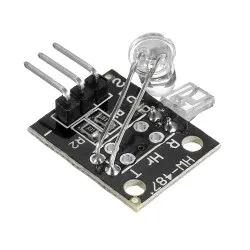
\includegraphics[scale = 0.5]{G21394} & \href{https://secure.sayal.com/STORE2/View_SHOP.php?SKU=247799}{Chaney Electronics Inc. G21394}  & Rejected & Due to the Infrared LED's Placement and the photoelectic sensor's placement, it is impossible to integrate the module with a device sitting on the wrist.\\
\hline
 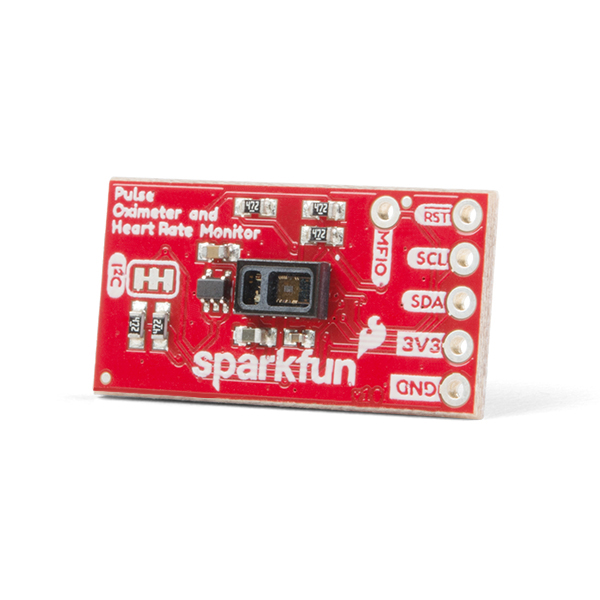
\includegraphics[scale = 0.5]{sparkfun} & \href{https://www.sparkfun.com/products/15219}{SparkFun Pulse Oximeter and Heart Rate Sensor - MAX30101 \& MAX32664 (Qwiic)}  & Rejected & Chronically out of stock, and requires extra complexity to be built into the PCB in order for this to function.\\
\hline
 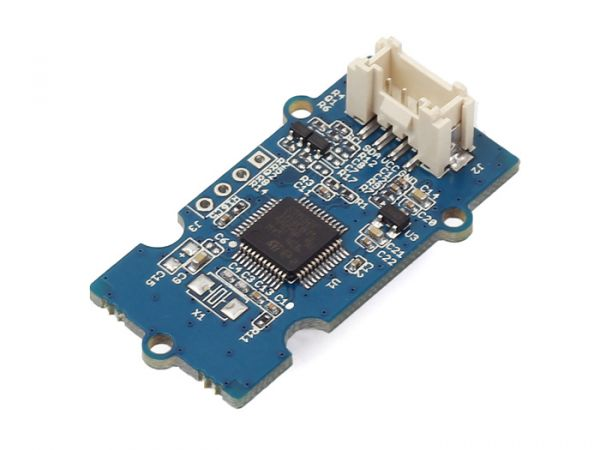
\includegraphics[scale = 0.25]{grove1} & \href{https://www.seeedstudio.com/Grove-Finger-clip-Heart-Rate-Sensor.html?queryID=ad9334e40c7058a87ffd810044eecd1c&objectID=711&indexName=bazaar_retailer_products}{Grove - Finger-clip Heart Rate Sensor}  & Rejected & Size too large, and issues with skin contact to the sensor results in garbage data.\\
\hline
 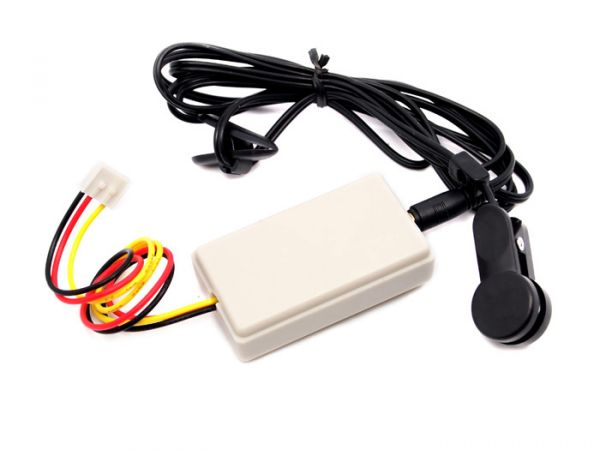
\includegraphics[scale = 0.25]{grove2} & \href{https://www.seeedstudio.com/Grove-Ear-clip-Heart-Rate-Sensor.html?queryID=ad9334e40c7058a87ffd810044eecd1c&objectID=2143&indexName=bazaar_retailer_products}{Grove - Ear-clip/Finger-clip Heart Rate Sensor}  & Rejected & Sensor attachment to the ear was considered too disruptive to the participant's daily activities.\\
\hline
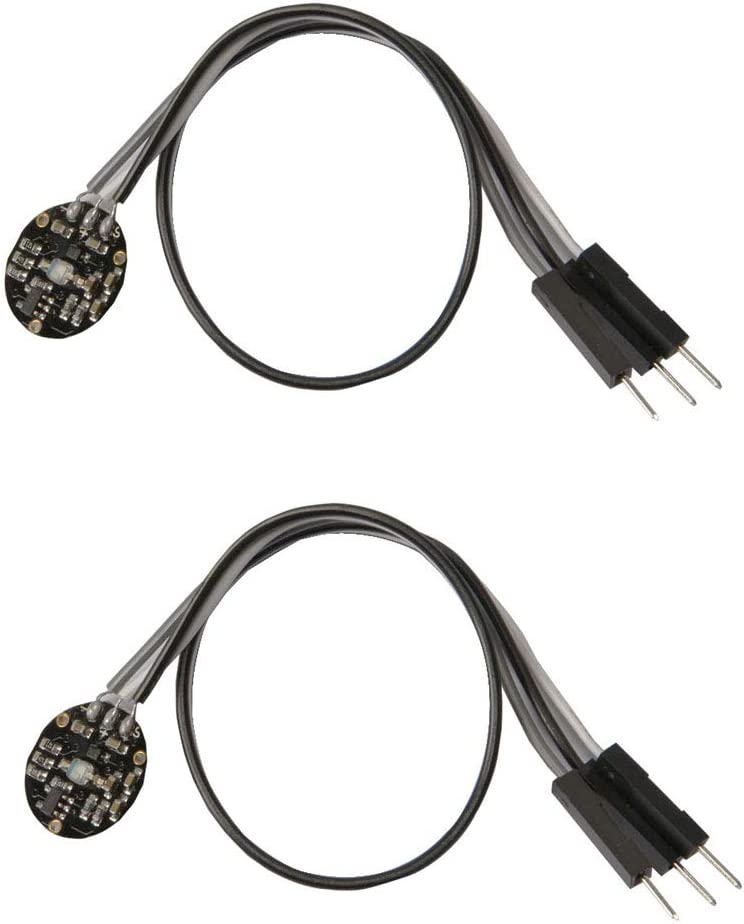
\includegraphics[scale = 0.1]{knockoff} & \href{https://www.amazon.ca/Comimark-Sensor-Module-Arduino-Raspberry/dp/B07V6VV8CM}{Comimark 2Pcs Heart Rate Pulse Sensor Sensor Module for Arduino Raspberry pi}  & Rejected & Build quality was unacceptably bad. Ordered name-brand version of this product next.\\
\hline

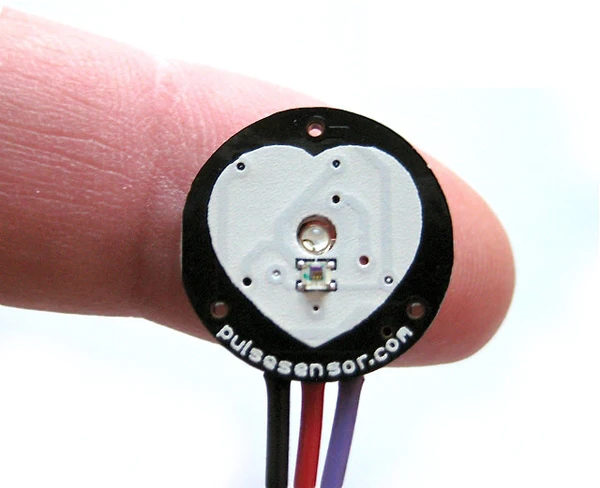
\includegraphics[scale = 0.25]{pulseSensor} & \href{https://pulsesensor.com/}{PulseSensor.com Pulse Sensor}  & Accepted & Build quality was better than knock-offs from before. Skin contact issue still present, but attempts are being made to solve this issue using software.\\
\hline
\end{tabular}
\end{table}

\section{Automated Testing}
N/A

\section{Trace to Requirements}
		
\section{Trace to Modules}		

\section{Code Coverage Metrics}

%\bibliographystyle{plainnat}
%\bibliography{../../refs/References}

\newpage{}
\section*{Appendix --- Reflection}

The information in this section will be used to evaluate the team members on the
graduate attribute of Reflection.  Please answer the following question:

\begin{enumerate}
  \item In what ways was the Verification and Validation (VnV) Plan different
  from the activities that were actually conducted for VnV?  If there were
  differences, what changes required the modification in the plan?  Why did
  these changes occur?  Would you be able to anticipate these changes in future
  projects?  If there weren't any differences, how was your team able to clearly
  predict a feasible amount of effort and the right tasks needed to build the
  evidence that demonstrates the required quality?  (It is expected that most
  teams will have had to deviate from their original VnV Plan.)
\end{enumerate}

\end{document}